\documentclass{article}

\usepackage{fancyhdr} % Required for custom headers
\usepackage{lastpage} % Required to determine the last page for the footer
\usepackage{extramarks} % Required for headers and footers
\usepackage[usenames,dvipsnames]{color} % Required for custom colors
\usepackage{graphicx} % Required to insert images
\usepackage{listings} % Required for insertion of code
\usepackage{courier} % Required for the courier font
\usepackage{lipsum} % Used for inserting dummy 'Lorem ipsum' text into the template
\usepackage{hyperref}
\usepackage{multirow}
\usepackage{tabularx}
\usepackage{longtable}
\usepackage{listings}
\usepackage{subfigure}
\usepackage{afterpage}
\usepackage{amsmath,amssymb}            
\usepackage{rotating}  
\usepackage{fancyhdr}
\usepackage{graphicx}
\usepackage{amsthm}
\usepackage[scriptsize]{caption} 
\hyphenation{a-gen-tiz-za-zio-ne}
% Margins
\topmargin=-0.45in
\evensidemargin=0in
\oddsidemargin=0in
\textwidth=6.5in
\textheight=9.0in
\headsep=0.25in

\linespread{1.1} % Line spacing

% Set up the header and footer
\pagestyle{fancy}
\lhead{\hmwkAuthorName} % Top left header
\chead{\hmwkClass\ (\hmwkClassInstructor\ \hmwkClassTime): \hmwkTitle} % Top center head
\rhead{\firstxmark} % Top right header
\lfoot{\lastxmark} % Bottom left footer
\cfoot{} % Bottom center footer
\rfoot{Page\ \thepage\ of\ \protect\pageref{LastPage}} % Bottom right footer
\renewcommand\headrulewidth{0.4pt} % Size of the header rule
\renewcommand\footrulewidth{0.4pt} % Size of the footer rule

\setlength\parindent{0pt} % Removes all indentation from paragraphs

\usepackage{listings}
\usepackage{color}

\definecolor{dkgreen}{rgb}{0,0.6,0}
\definecolor{gray}{rgb}{0.5,0.5,0.5}
\definecolor{mauve}{rgb}{0.58,0,0.82}

\lstset{frame=tb,
  language=Java,
  aboveskip=3mm,
  belowskip=3mm,
  showstringspaces=false,
  columns=flexible,
  basicstyle={\small\ttfamily},
  numbers=none,
  numberstyle=\tiny\color{gray},
  keywordstyle=\color{blue},
  commentstyle=\color{dkgreen},
  stringstyle=\color{mauve},
  breaklines=true,
  breakatwhitespace=true
  tabsize=3
}

%----------------------------------------------------------------------------------------
%	DOCUMENT STRUCTURE COMMANDS
%	Skip this unless you know what you're doing
%----------------------------------------------------------------------------------------

% Header and footer for when a page split occurs within a problem environment
\newcommand{\enterProblemHeader}[1]{
\nobreak\extramarks{#1}{#1 continued on next page\ldots}\nobreak
\nobreak\extramarks{#1 (continued)}{#1 continued on next page\ldots}\nobreak
}

% Header and footer for when a page split occurs between problem environments
\newcommand{\exitProblemHeader}[1]{
\nobreak\extramarks{#1 (continued)}{#1 continued on next page\ldots}\nobreak
\nobreak\extramarks{#1}{}\nobreak
}




%----------------------------------------------------------------------------------------
%	NAME AND CLASS SECTION
%----------------------------------------------------------------------------------------

\newcommand{\hmwkTitle}{Design Pattern} % Assignment title
\newcommand{\hmwkDueDate}{Martedi,\ Aprile 15,\ 2014} % Due date
\newcommand{\hmwkClass}{Ingegneria del Software 1} % Course/class
\newcommand{\hmwkClassTime}{} % Class/lecture time
\newcommand{\hmwkClassInstructor}{} % Teacher/lecturer
\newcommand{\hmwkAuthorName}{} % Your name

%----------------------------------------------------------------------------------------
%	TITLE PAGE
%----------------------------------------------------------------------------------------

\title{
\vspace{2in}
\textmd{\textbf{\hmwkClass:\ \hmwkTitle}}\\
\normalsize\vspace{0.1in}\small{Due\ on\ \hmwkDueDate}\\
\vspace{0.1in}\large{\textit{\hmwkClassInstructor\ \hmwkClassTime}}
\vspace{3in}
}

\author{\textbf{\hmwkAuthorName}}
\date{} % Insert date here if you want it to appear below your name

%----------------------------------------------------------------------------------------

\begin{document}

\maketitle

%----------------------------------------------------------------------------------------
%	TABLE OF CONTENTS
%----------------------------------------------------------------------------------------

%\setcounter{tocdepth}{1} % Uncomment this line if you don't want subsections listed in the ToC

\newpage
\tableofcontents
\newpage



%----------------------------------------------------------------------------------------
\section{Introduction}


\section{Creational Patterns}
Inside the class of the creational patterns we can distinguish between two main pattern:
\begin{itemize}
\item \textbf{class creational pattern} uses inheritance to change how the different classes are intantiated.
\item \textbf{object creational pattern} delegate the instantiation of the object to another object.
\end{itemize}
The object creational pattern become important when it is necessary to compose a smaller set of composed behavior into complex one. Thus, creating an object with a particular behavior is more complex then simply instantiating a new class.

\subsection{Prototype}

\subsection{Abstract Factory (Kit)}
\subsubsection{Goal}
The goal is to create an interface which allows \textbf{to create families} of related or dependent objects, \textit{without specifying} their concrete classes. 

\subsubsection{Structure}

\begin{figure}[h!]
  \centering
    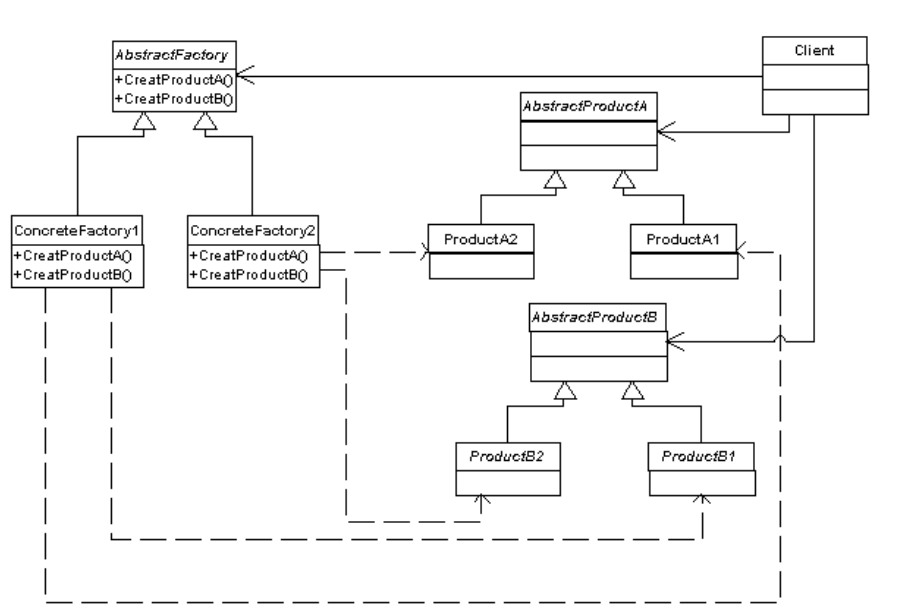
\includegraphics[width=0.8\textwidth]{Img/AbstractFactoryUML.png}
     \caption{Abstract Factory UML.}
     \label{AbstractFactoryUML}
\end{figure}

Using this pattern an abstract framework (factory) is defined, which allows to create objects that follow a general pattern. At run-time the abstract factory is paired with any concrete factory that allows to create the objects that follow the concrete pattern. In other words, the Abstract Factory is a super-factory which creates other factories (Factory of factories). The UML of Figure~\ref{AbstractFactoryUML} is composed by the following classes:
\begin{itemize}
\item \emph{AbstractFactory}: is an abstract class (see the italic style of the text), which declares the interface for the operations that allows to create \emph{abstract} products
\item \emph{ConcreteFactory}: are the concrete classes that allows to create \emph{concrete} products (Note the hierarchical relation between the AbstractFactory and the ConcreteFactory). Each product is a family of related dependent objects AbstractProductA and AbstractProductB, and in particular, for the ConcreteFactory1 the products are ProductA1 and ProductB1, while for the ConcreteFactory2 the products are ProductA2 and ProductB2 (Note the uses relation between the Factories and the products).
\item \emph{AbstractProduct}:  declares an abstract product which can be aggregated to other products using appropriate factories
\item \emph{ConcreteProduct}: are  concrete products which extends  particular abstract products.
\item \emph{Client}: instantiate a specific ConcreteFactory (depending on its necessities) to obtain specific products.
\end{itemize}

Note: usually only a single instance of a ConcreteFactory class is created at run-time. The AbstractFactory defers the creation of products to the ConcreteFactories.

\subsubsection{Examples}
\textbf{Window Interface}\\
Consider a user interface that must support multiple devices, such as laptops, cellphones. Different interfaces must be creating depending on the device which runs the application (e.g., different type of scroll bars, windows, buttons). To be portable, the application should not be hard-coded to a particular look and feel. The instantiation and the designing new look-and-feels must be easy. The example is inspired by~\cite{gamma1994design}.


\subsubsection{Implementation}
\begin{itemize}
\item \emph{AbstractFactory} only declare the interface for the creating the products
\item \emph{ConcreteFactory} are \emph{singleton}. A \emph{factory method} is defined for each product. 

\end{itemize}

\subsubsection{Pro and Cons}
\begin{itemize}
\item it requires a concrete factory subclass for each product even if the families differ only slightly
\item if many families are possible think about using a \emph{prototype pattern} inside the factory (You can store classes inside a concrete factory that create the various concrete products in variables, much like prototypes).
\item AbstractFactory usually define a \emph{different operation} for each kind of product it is possible to create, i.e., for each product there is a signature in the AbstractFactory Interface. This implies that \emph{to add a new product} you must add the \emph{signature in the abstract factory} and all the sub Factory-classes. A \textbf{more flexible} but \textbf{less safe} design is to add a parameter in the operations to create objects. This parameter specifies the object to be created (e.g., an enum).
\item All the products are returned to the client as abstract interfaces to the product. The client is not able to make safe assumption on the type of the product.
\end{itemize}


\subsection{Builder}
\subsubsection{Goal}
Separate the construction of a complex object from its representation, so that the same construction process can create different representations.

\subsubsection{Motivation}

\subsection{Singleton}

\subsection{Factory Method (Virtual Constructor)}
\subsubsection{Goal}
Define an interface for creating an object, but let sub-classes decide which class to instantiate.

\clearpage
% ---- Bibliography ----




\addcontentsline{toc}{chapter}{Bibliography}
\bibliographystyle{alpha}
\bibliography{DesignPatterns}
\nocite{*}


\end{document}

